_A Motorstatus liefern
_C n konstante Geschwindigkeit einstellen
_D n Bezugswert definieren
_E nMotorstrom einstellen
_F Standardeinstellungen aktivieren
_H Sanfter stop
_I 4-Bit-Eingang lesen
_J jdss Joystickparameter einstellen
_L n lokalen Modus aktivieren/beenden
_M n n Schritte ausführen
_MA n zu n bewegen
_MC n mit konstanter Geschwindigkeit bewegen
_MCA n MAmit konstanter Geschwindigkeit
_MCL n MC zu Endschalterposition
_ML n zur Endschalterposition bewegen
_N n Zeilenvorschub (LF, hex. 0A) einfügen/löschen
_O n n an 4-Bit-Ausgang senden
_P nnnn Motorparameter einstellen
_Q Parameter in EEROM speichern
_R n Mikroschritteilung einstellen
_RL Endschalterwerte lesen
_RS verbleibende Schritte lesen
_S Nothalt
_T n Eingang n auslösen
_W Position anfordern

\begin{longtable}{|m{10cm}|m{3cm}|}
\caption{Elemente der Ereignisgesteuerten Prozesskette} \\
\hline
\label{tab:ElementeDerEreignisgesteuertenProzesskette}
\textbf{Element} & \textbf{Symbol}\\
\hline
\textbf{Funktion} 

Funktionen beschreiben Tätigkeiten, die im Verlauf des Geschäftsprozesses anfallen. Sie können von Mitarbeitern oder einem Informationssystem durchgeführt werden und benötigen evtl. Ressourcen, die ihnen zugewiesen werden. 

Beispiele: \textit{Auftrag anlegen}, \textit{Rechnung schreiben}, \textit{Konto abschließen} & 
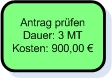
\includegraphics[width=3cm]{EPK-Funktion.jpg} \\
\hline
\textbf{Ereignis} 

Ereignisse sind betriebswirtschaftlich relevante Ereignisse, die den Geschäftsprozess in irgendeiner Weise steuern oder beeinflussen. Ereignisse sind immer Auslöser oder Ergebnisse von Funktionen. Ein Geschäftsprozess beginnt und endet stets mit einem Ereignis. 

Beispiele: \textit{Auftrag eingetroffen}, \textit{Überweisung getätigt}, \textit{Rechnung erstellt} & 
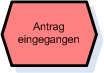
\includegraphics[width=3cm]{EPK-Ereignis.jpg} \\
\hline
\textbf{Operatoren} 

Operatoren steuern den Kontrollfluss eines Geschäftsprozesses. Sie machen \zB deutlich, dass eine Funktion mehrere Ereignisse auslöst, oder zeigen alternative Vorgehensweisen an. Es gibt drei Operatoren (v.\,l.\,n.\,r.\,): UND, ODER und XODER (exklusives ODER). & 

\includegraphics[width=3cm]{EPK-Operatoren.jpg} \\
\hline
\textbf{Organisationseinheit} 

Organisationseinheiten werden Funktionen zugeordnet und beschreiben, wo die Funktionen ausgeführt werden bzw. wer sie ausführt. Die Bezeichnung der Symbole enthält zusätzlich zur Abteilung noch die Namen der Mitarbeiter.

Beispiele: \textit{Vertrieb}, \textit{Personal}, \textit{Produktion} & 
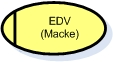
\includegraphics[width=3cm]{EPK-Organisationseinheit.jpg} \\
\hline
\textbf{Informationsobjekt} 

Auch Informationsobjekte werden Funktionen zugewiesen und beschreiben die von diesen benötigten oder erstellten Informationen. Dabei sind sämtliche Formen von Informationen auf verschiedenen Datenträgern möglich und nicht etwa nur digitale Daten. Die Bezeichnung der Symbole enthält zusätzlich das Informationssystem, aus dem die Informationen stammen.

Beispiele: \textit{Kundendatenbank}, \textit{Versicherungsantrag}, \textit{Rechnung} & 
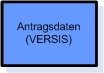
\includegraphics[width=3cm]{EPK-Informationen.jpg} \\
\hline
\textbf{Prozesswegweiser}

Mit Prozesswegweisern werden Prozesse, die in anderen EPKs beschrieben sind, referenziert. So können \zB unübersichtliche Prozesse in Teilprozesse gegliedert und häufig verwendete Prozesse an zentraler Stelle modelliert werden. Prozesswegweiser stehen in einer EPK immer anstelle von Funktionen. & 
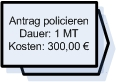
\includegraphics[width=3cm]{EPK-Prozesspfad.jpg} \\
\hline
\end{longtable}
